\documentclass{article}


\usepackage{arxiv}

\usepackage[utf8]{inputenc} % allow utf-8 input
\usepackage[T1]{fontenc}    % use 8-bit T1 fonts
\usepackage{url}            % simple URL typesetting
\usepackage{booktabs}       % professional-quality tables
\usepackage{amsfonts}       % blackboard math symbols
\usepackage{amsmath}
\usepackage{nicefrac}       % compact symbols for 1/2, etc.
\usepackage{microtype}      % microtypography
\usepackage{xcolor}
\usepackage{lipsum}
\usepackage{graphicx}
\usepackage{pslatex}
\usepackage{apacite}
\usepackage{natbib}
\usepackage{lineno}
\usepackage{prettyref}
\usepackage{hyperref}
\usepackage{rotating}  % For sidewaysfigure
\usepackage{graphicx}
\graphicspath{ {../gfx/} 
% \graphicspath{ {./figures/}

% Prettyref Configuration
\newrefformat{cap}{Figure~\ref{#1}}
\newrefformat{fig}{Figure~\ref{#1}}
\newrefformat{tab}{Table~\ref{#1}}
\newrefformat{sec}{Section~\ref{#1}}
\newrefformat{sub}{Section~\ref{#1}}
\newrefformat{subsec}{Section~\ref{#1}}
\newrefformat{cha}{Chapter~\ref{#1}}
\newrefformat{lis}{Listing~\ref{#1}}
\newrefformat{eq}{Eq.~\ref{#1}}

\title{DynVision: \\A Toolbox for Biologically Plausible Recurrent Convolutional Networks}

\author{
Robin Gutzen \\
Center for Data Science \\ 
New York University \\ 
New York, USA \\
\texttt{robin.gutzen@nyu.edu} \\
   \And
Grace W Lindsay \\
Center for Data Science and Department of Psychology \\ 
New York University \\ 
New York, USA \\
\texttt{gm3239@nyu.edu} \\
}

\begin{document}
\maketitle
\begin{abstract}
% Paragraph 1: Problem statement - Current limitations in modeling biological temporal dynamics in vision systems, lack of accessible tools for continuous-time recurrent models, citing the gap between discrete-time approaches (Kietzmann et al. 2019) and continuous neural dynamics (Groen et al. 2022).
% Paragraph 2: Solution overview - Introduce DynVision as a comprehensive toolbox bridging neuroscience and deep learning, emphasizing modular architecture and biological plausibility inspired by frameworks like ORGaNICs (Heeger & Mackey 2019) and CORnet (Kubilius et al. 2019).
% Paragraph 3: Key capabilities - Highlight continuous dynamics with heterogeneous delays, multiple recurrence types, workflow integration, and performance optimizations achieving 52% speedup over reference implementations.
% Paragraph 4: Demonstration results - Mention systematic comparison of recurrence types showing distinct temporal characteristics, biological validation against cortical recordings (following Groen et al. 2022), and novel insights about subadditive temporal summation.
% Paragraph 5: Impact statement - Conclude with the toolbox's potential to accelerate research in computational neuroscience and biologically inspired AI, democratizing access to continuous-time neural modeling.
Convolutional Neural Networks (CNNs) have demonstrated remarkable success in image recognition and exhibit conceptual similarities to the primate ventral visual pathway. Adding recurrence opens the door to exploring temporal dynamics and investigating mechanisms underlying recognition robustness, attentional modulation, and rhythmic perception phenomena. However, modeling spatiotemporal dynamics of biological vision using CNN-based architectures remains challenging. Incorporating functionally beneficial recurrence, capturing biologically plausible temporal phenomena such as adaptation and subadditive temporal summation, and maintaining topographic organization aligned with cortical structure require significant computational considerations. Although recent advances have incorporated neurobiological constraints, the field lacks accessible tools for efficiently integrating, testing, and comparing these approaches.
Here, we introduce DynVision, a modular toolbox for constructing and evaluating recurrent convolutional neural networks (RCNNs) with biologically inspired dynamics. Our approach facilitates the incorporation of key visual cortex properties, including realistic recurrent architectures, activity evolution governed by dynamical systems equations, and structured connectivity reflecting cortical arrangements, while maintaining computational efficiency. We demonstrate the framework's utility through systematic analysis of emergent neural dynamics, highlighting how different biologically motivated modifications shape scientifically-relevant response patterns. Code can be found at: \url{https://github.com/Lindsay-Lab/DynVision/}
% All results are reproducible from scratch, including model training, on a compute cluster with gpu cores within a day.
\end{abstract}


% keywords can be removed
%\keywords{First keyword \and Second keyword \and More}

\section{Introduction} 
% \subsection*{\textit{Motivation: The Need for Biologically Plausible Temporal Dynamics}}
% Comment: This subsection establishes the scientific foundation by explaining why current approaches are insufficient and why biological plausibility matters for vision research. The argument should flow from biological evidence to computational limitations to research needs.
The primate visual system is characterized by abundant recurrent connections \cite{vanBergen2020_176}. In the ventral visual stream, for example, lateral recurrent connections exist amongst neurons within a visual cortical region and feedback connections go from higher areas like V4 back to lower ones such as V1. These connections are believed to play a crucial role in the system's remarkable ability to integrate information over time and recognize objects under diverse viewing conditions and with varying degrees of occlusion or noise. %[TODO: CITES]. 

%Notably, the visual system also features extensive recurrent connections that are yet missing in many computer vision models. 


For these reasons, many researchers have attempted to integrate these connections into one of the leading classes of visual system models: convolutional neural networks \citep{Lindsay2021_2017}. Although many past studies on recurrent convolutional neural networks (RCNNs) have found benefits of adding recurrence \cite{Kietzmann2019_21854, Spoerer2020_e1008215, Kar2019_974}, others have had mixed results or found that recurrence does not serve the same function as in the brain \cite{Maniquet2024_, Nayebi2022_1652, Lindsay2022_a}. 

% Paragraph 1: Biological evidence for temporal dynamics in vision - Cite evidence from Groen et al. 2022 showing cortical temporal responses with adaptation and subadditive summation, van Bergen & Kriegeskorte 2020 review of recurrent processing in primate visual system, and Ohki et al. 2006 on cortical topographic organization.
% Paragraph 2: Limitations of standard CNNs - Explain how feedforward architectures miss crucial temporal dynamics, cite Lindsay 2021 review, mention inability to capture phenomena like adaptation, contextual modulation, and temporal integration that are fundamental to biological vision.
% Paragraph 3: Problems with existing RCNN approaches - Discuss limitations of discrete-time models (Kietzmann et al. 2019, Spoerer et al. 2020), coarse temporal approximations missing fine-grained dynamics, and mixed results in literature (Maniquet et al. 2024, Nayebi et al. 2022) suggesting need for better temporal modeling.
% Paragraph 4: Engineering challenges - Describe computational difficulties in implementing continuous-time models, memory requirements for long sequences, gradient flow through time, and lack of accessible tools for systematic exploration of biological constraints.
% Paragraph 5: Research gap identification - Emphasize the need for accessible tools that enable systematic exploration of biologically plausible architectures while maintaining computational efficiency, referencing successful approaches in ORGaNICs (Heeger & Mackey 2019) and Neural ODEs (Chen et al. 2018).

% \subsection*{\textit{Existing Approaches and Their Limitations}}
% Comment: This subsection provides a comprehensive review of related work, positioning DynVision relative to existing solutions. The tone should be balanced, acknowledging contributions while identifying gaps.
%While recurrent connections are ubiquitous in primate visual system, their integration into computer vision models is more elusive both in terms of being functionally beneficial and computationally efficent \cite{Maniquet2024, Kar2019}. Recurrent computations involve iterative processing, which can significantly increase the time and energy required for inference compared to feedforward networks. 
%Still there many promising approaches in that regard. \citet{} showed that recurrent convolutional neural networks (RCNNs) can exhibit flexible trading of speed for accuracy, and reaction times that correlated well with human reaction times for the same images. \citet{Nayebi2022} found that standard recurrent networks (RNNs and LSTMs) did not improve performance on ImageNet classification. However, innovative cells incorporating bypassing and gating mechanisms significantly boosted accuracy, highlighting the importance of designing specialized recurrent units inspired by the neuroanatomy of the ventral visual stream \cite{Zhang2024, Toosi2023, ...}.

% much of the current work on CNN - visual cortex similarity focuses on the representational similarites between the systems. With some work looking more into the topographic organization

These studies predominantly use discrete-time recurrent models, usually unrolled for only a handful of time steps. This coarse-grain approximation to recurrence cannot capture the full complexity of visual dynamics, and it may make it difficult for the network to learn the right parameters that replicate biology. The discrete-time approach is also at odds with more traditional methods in computational neuroscience, which treat neural circuits as continuous dynamical systems governed by differential equations.

Using continuous-time models in a machine learning setting poses certain engineering challenges. Specifically, neural dynamics are best captured using a small simulation step size (on the order of one millisecond), which requires tens to hundreds of time steps to mimic the visual system's response. This leads to a large computational graph when training with back-propagation through time. The implementation of these networks must therefore be made as efficient as possible to make exploration of relevant scientific questions with them feasible. Here, inspired by recent work that combines continuous-time differential equations with deep convolutional neural networks \citep{Soo2024_, Heeger2019_22783, Lindsay2020_2019.12.13.875534}, we build a toolbox to make the use of such models easier and more widely available.   

% focus on scientific questions rather than implementation details.


% Paragraph 1: Review of discrete-time RCNN frameworks - Discuss CORnet family (Kubilius et al. 2019, Schrimpf et al. 2020), VOneNet extensions (Dapello et al. 2020), ReAlnet-fMRI (Lu & Wang 2024), their achievements in Brain-Score optimization but limitations in temporal precision.
% Paragraph 2: Continuous-time neural frameworks - Compare with Neural ODEs (Chen et al. 2018), Liquid Time-Constant Networks (Hasani et al. 2022), Neural Delay Differential Equations (Oprea et al. 2023, Zhu et al. 2023), their theoretical elegance but limited application to vision tasks.
% Paragraph 3: Computational neuroscience simulation tools - Review BRIAN2, NEST, their strengths in detailed neural modeling but limitations for large-scale vision tasks, lack of integration with modern deep learning infrastructure, and computational overhead.
% Paragraph 4: Unified theoretical frameworks - Discuss ORGaNICs framework (Heeger & Mackey 2019) for oscillatory dynamics, Brain-Like Transformers (spike-driven transformers, neuron-astrocyte attention), their theoretical contributions but limited practical implementation for vision research.
% Paragraph 5: Gap analysis - Synthesize the need for a tool that combines biological realism of neuroscience simulators, computational efficiency of deep learning frameworks, systematic experimentation capabilities, and modern ML infrastructure integration.

% \subsection*{\textit{DynVision: A Toolbox Solution}}
% Comment: This subsection introduces DynVision as the solution to identified problems. The presentation should be confident but not overselling, focusing on concrete capabilities and design decisions.
Our toolbox, DynVision, implements numerical ODE solvers to build RCNNs with more precise and realistic temporal dynamics. It allows for many different forms of recurrent connections, with options that are inspired by biology and that can help with efficiency. Users can also control a variety of parameters that govern dynamics within and across regions. Synthesizing approaches from the literature, we also include retina-inspired pre-processing, optional gain modulation, and activity regularization. We hope that providing this toolbox will help the community iterate on models of dynamical visual processing faster and more broadly.

% Paragraph 1: Core philosophy - Explain the design principle of bridging computational neuroscience and deep learning, emphasizing systematic experimentation and reproducibility, inspired by successful frameworks like CORnet's modular approach and ORGaNICs' biological realism.
% Paragraph 2: Key technical innovations - Introduce continuous-time dynamics with heterogeneous delays, modular recurrence types (self, full, depthwise, local), biological constraint integration (supralinear activations, energy losses), and topographic organization support.
% Paragraph 3: Software engineering approach - Describe integration with PyTorch Lightning for training infrastructure, Snakemake for workflow management, FFCV for data optimization, configuration-driven design, and modern ML practices enabling reproducible research.
% Paragraph 4: Target applications - Define use cases for computational neuroscientists studying visual processing, AI researchers exploring biological architectures, vision scientists validating models against neural data, and researchers investigating temporal dynamics in perception.
% Paragraph 5: Paper overview - Preview the structure of the paper, emphasizing both technical description and scientific demonstrations, systematic comparison with existing frameworks, and novel insights about temporal dynamics in vision.

% \begin{figure}[ht]
% \begin{center}
% % \includegraphics[width=\linewidth]{figures/dynvision_overview.pdf}
% \end{center}
% \caption{\textbf{DynVision bridges computational neuroscience and deep learning.} Conceptual diagram showing how DynVision fills the gap between traditional CNNs (left) and biological neural networks (right) by incorporating continuous temporal dynamics, heterogeneous delays, and biologically plausible connectivity patterns while maintaining computational efficiency and modern ML infrastructure integration.}
% \label{fig:dynvision_overview}
% \end{figure}

\section{Toolbox Design and Implementation}
Here, we provide a description of the overarching philosophy and core functionalities of the DynVision toolbox. For a more detailed account of all functionalities, consult the DynVision software documentation. Code can be found at: \url{https://github.com/Lindsay-Lab/DynVision/}.

\subsection{Design Approach}
% Comment: This subsection explains the high-level design decisions that make DynVision unique. The argument should connect design choices to scientific goals and usability requirements.

\paragraph{Abstraction Level}
% Paragraph 1: Biological abstraction levels - Describe the choice to focus on rate-based dynamics rather than spiking models, balancing biological plausibility with computational tractability, learning from Neural ODEs' success in continuous-time modeling and ORGaNICs' unified framework approach.
On the one end of the computational neuroscience modeling spectrum there are detailed neural networks involving morphologies, cell-types, and spikes that focus on simulating realistic neural activity (e.g. NEST, Neuron, BRIAN). On the other end, there are abstract network models often based on machine learning methodologies that focus on learning and optimized behavioral performance such as classification (e.g. VGG, ResNet, Transformers). Complementary to the modeling efforts on either extreme, NeuroAI models (for lack of a better term) focus on information processing with biologically plausible dynamics at a level of abstraction that enables both computational ability and meaningful comparison with neural data and behavioral data.
DynVision supports this modeling niche wherein biological realism and performance optimization are both required for the purposes of studying how biological features give rise to behavior. 

\paragraph{Biological Analogies}
% conv and pool operation : connections between (pyramidal) neuron populations
% non-linearity: action potential creation
% dynamics step: membrane potential
% hidden states: conduction delays
% integration of reccurent activity: connections via interneurons
% integration of skip and feedback activity: connection between neuron populations of different cortical areas (gain control)
% the biological anlogies can greatly inform the network architecture by taking the morphologies and connectivity paradigms in the cortex as a guide
Components of an artificial neural network can be mapped to biology in a variety of ways and with varying levels of specificity. Multi-layer CNNs, for example, parallel the hierarchical compositionality of the ventral visual stream (V1 -> V2 -> V4 -> IT), with early layers detecting simple features through small receptive fields analogous to V1 simple with additional pooling operations representing the function of complex cells \citep{Lindsay2021_2017}. Deeper layers progressively combine these features into increasingly abstract representations and larger receptive fields. Weight sharing and spatial pooling in CNN models realize a translational invariance that support the learning of generalizable visual features and  the recognition of objects regardless of their precise position. The convolutional tensor operations maintain a spatial correspondence of the visual field, representing the retinotopic organization found in the visual cortex.

On the smaller scale, we here interpret each entry in the 3D activation tensor ([\verb|n_channels, y_dim, x_dim|]) as a unit representative of a single neuron or a population of neurons, with the activation value corresponding to an average spiking rate. This interpretation establishes direct correspondences between network components and cortical structures: convolutional operations represent connections between pyramidal neuron populations within or between cortical layers, pooling operations mimic the behavior of complex cells in\citep{Lindsay2021_2017}, while non-linearities model the mechanism of action potential generation, and the dynamical systems formulation captures membrane potential dynamics. %todo: do we need cites for these things?

The hidden states hold several timesteps of activity; accessing different timestep slots in the hidden states can represent the conduction delays that can vary across connection types (see Figure \ref{fig:layer_ordering}). Recurrent connections communicate delayed activity within a cortical area, potentially mediated by interneuron populations. Skip and feedback connections represent inter-areal communication between hierarchical cortical regions (e.g., V4->V1 feedback). These biological analogies actively inform architectural choices, as cortical morphology and connectivity paradigms constrain the network design space. Building off these analogies, we believe that more biologically plausible recurrent convolutional networks may capture aspects of human visual behavior and its computational efficiency.

%\subsubsection{Biological Analogies of CNN Connections}
% biologial motivation for recurrence and realization via convolutions + up/down sampling operations and storing of hidden states
%CNN architectures have shown a surprising effectiveness in computer vision applications \citep{?}. There effectiveness is thought to stem from CNNs mirroring several core paradigms of organizational principles of the primate visual system.
%\paragraph{Biological Analogies of Temporal Parameters}
% Paragraph 4: Explain the biological interpretation of $\tau$, typical values from literature (10-50 ms range from cortical recordings), and impact on model dynamics, referencing Groen et al. 2022 temporal response measurements.
% Paragraph 5: Performance considerations - Describe the approach to maintaining computational efficiency while adding biological constraints, including optimization strategies inspired by FFCV dataloader improvements and hardware utilization techniques from Neural ODEs literature.
% merge with 'Performance Optimizations' subsection!? 

In the following sections we provide an overview of the options our toolbox provides to users, motivated by what is needed in order to efficiently explore biologically-inspired dynamics. 



\begin{figure}[ht]
\begin{center}
\includegraphics[width=1\linewidth]{rcnn_architecture.png}
\end{center}
\caption{\textbf{Architecture schematic of the DyRCNN model family, native to the DynVision toolbox.}
The left hand side shows the signal flow and processing within one network layer. The layer operations are shown as circular pictograms or the merging or splitting of arrows. The layer units are represented by their 3D activation tensors.
The order of layer operations (vertical labels) can be flexibly arranged as described in \ref{sec:layer_operations}. Recurrent activity can be integrated with the `input' (shown here), `middle', or `output' activations of the convolutions.
Pointers to specific timestep slots of the hidden state indicate the respective delays (\ref{sub:delays}), here $\Delta_{FF}=2$, $\Delta_{RC}=2$, $\Delta_{FB}=2$, $\Delta_{SK}=4$. 
The right hand side shows our four-layer network, the layer parameters, and the connections between layers. Note that the pooling operation is only applied in V1 and V2. The tuple parameters indicate the individual values for the two convolutions in the respective layer, when they differ from each other.
}
\label{fig:layer_ordering}
\end{figure}

\subsection{Temporal Dynamics}
% Comment: This subsection provides the mathematical foundation for the time dynamics. Equations should be clearly presented with biological interpretations and implementation details.

\paragraph{Dynamical System Network Description}
% Paragraph 1: Continuous-time dynamics equation - Present the core differential equation with detailed explanation of each term and its biological significance, connecting to ORGaNICs framework and Neural ODEs literature.
In biological neural networks, activity evolves over time and space in a structured and continuous manner, based on past input and intrinsic network properties. DynVision implements numerical ODE solvers to build RCNNs with more precise and realistic temporal dynamics. 
This is often modeled within a dynamical system formulation as the differential equation in \prettyref{fig:dynamical_systems_equation} (1) 
\citep{Heeger2019_22783, Soo2024_}. 
The toolbox incorporates this dynamical systems formulation by accordingly evolving the activity over time using a stepwise numerical differential equation solver (Euler method, \prettyref{fig:dynamical_systems_equation} (2)), which evolves a layer's activity on a timescale $\tau$ for the next time step $t$ based on the layer's activity of the previous timestep $t-dt$ and any input to this layer arriving at that timestep.

Note that some details of this formalism can modified by reordering the order of operations that are executed for each layer (with the \verb|layer_operations| list parameter; see \ref{sec:layer_operations}). This can include placing certain inputs outside of the activation function or moving the bias outside of the temporal evolution step.

\paragraph{Heterogeneous Delays} \label{sub:delays}
% Paragraph 3: Heterogeneous delay implementation - Describe how different connection types (feedforward, recurrent, feedback) can have distinct propagation delays reflecting biological conduction velocities, inspired by Neural Delay Differential Equations (Oprea et al. 2023, Zhu et al. 2023).
Different neural connections are governed by different temporal delays, reflecting conduction velocities and the spatial distance between the neurons. 
Our toolbox allows for temporal unrolling with separate time delays for different types of connections between network layers. Specifically, at time $t$ a layer can receive input from its own past activity $r_l$ at $t-\Delta_{RC}$ via the laterally recurrent connections $J_{RC}$, feedforward input from the preceding layer $r_{l-1}$ at $t-\Delta_{FF}$ via the connectivity $J_{FF}$, and recurrent feedback connections from a succeeding layer $r_{>l}$ via $J_{FB}$.
By varying these parameters, users can systematically evaluate the influence of different temporal delays on network dynamics. 

\begin{figure}[ht!]
\begin{flushleft}
% Define the colors to match the SVG
\definecolor{red}{HTML}{c4380f}      % Dynamical Timescale
\definecolor{blue}{HTML}{18359c}     % Network Activations  
\definecolor{gray}{HTML}{5f5b5b}     % Time Dimension
\definecolor{purple}{HTML}{821ca9}   % Non-linearity
\definecolor{teal}{HTML}{17a89c}     % Network Connectivity
\definecolor{green}{HTML}{41960e}    % External (LFP) Input
\definecolor{orange}{HTML}{b8621a}   % Time Step
\definecolor{olive}{HTML}{556B2F}  % Bias

\newcommand{\annotsize}{\tiny}

\begin{align}
&\notag\hspace{-0.8cm}
{\color{red}\text{\annotsize{Dynamical\ Timescale}}} \hspace{0.2cm} 
{\color{blue}\text{\annotsize{Network\ Activations}}} \hspace{0.2cm} 
{\color{green}\text{\annotsize{External\ Input}}} \hspace{0.2cm} 
{\color{olive}\text{\annotsize{Bias}}}\\
&{\color{red}\tau} \frac{d{\color{blue}r}}{d{\color{gray}t}} = -{\color{blue}r}({\color{gray}t}) + {\color{purple}\Phi}{\color{purple}\left[}{\color{black}{\color{green}I}({\color{gray}t}) + {\color{teal}J}{\color{blue}r}({\color{gray}t})}{\color{purple}\right]} + {\color{olive}B}\\
&\notag\hspace{-0.3cm}
{\color{gray}\text{\annotsize{Time\ Dimension}}} \hspace{0.2cm} 
{\color{purple}\text{\annotsize{Activation\ Function}}} \hspace{0.2cm} 
{\color{teal}\text{\annotsize{Network\ Connectivity}}} \hspace{0.2cm} 
{\color{orange}\text{\annotsize{Time\ Step/Delay}}}\\
&{\color{blue}r_l}({\color{gray}t}) = {\color{blue}r_l}({\color{gray}t}-{\color{orange}dt}) + \frac{{\color{orange}dt}}{\color{red}\tau} \left(-{\color{blue}r_l}({\color{gray}t}-{\color{orange}dt}) + {\color{purple}\Phi}{\color{purple}\left[}{\color{black}{\color{green}I_l}({\color{gray}t}-{\color{orange}dt}) + \sum_{s=0}^{{\color{gray}t}-{\color{orange}dt}} {\color{teal}J_l} {\color{blue}r}({\color{gray}s}){\color{purple}\right]}}+ {\color{olive}B_l}\right)\\
&\sum_{{\color{gray}s}=0}^{{\color{gray}t}-{\color{orange}dt}} {\color{teal}J_l} {\color{blue}r}({\color{gray}s}) = 
{\color{teal}J_{FF}}\cdot {\color{blue}r_{l-1}}({\color{gray}t}-{\color{orange}\Delta_{FF}}) + 
{\color{teal}J_{RC}}\cdot {\color{blue}r_l}({\color{gray}t}-{\color{orange}\Delta_{RC}}) + 
{\color{teal}J_{FB}}\cdot {\color{blue}r_{>l}}({\color{gray}t}-{\color{orange}\Delta_{FB}}) + 
{\color{teal}J_{SK}}\cdot {\color{blue}r_{<l-1}}({\color{gray}t}-{\color{orange}\Delta_{SK}})
\end{align}
\caption{\textbf{Dynamical systems formulation of the neural network activity with heterogenous connectivity and delays.} \textbf{1)} Differential equation describing the evolution of network activity over time given the connectivity, and input, with a timescale given by $\tau$. \textbf{2)} A numerical stepwise approach to approximately solving the differential equation via the Euler method for the activity $r_l$ in layer $l$ for the subsequent time step $t$. The contributions by feedforward (FF), lateral recurrent (RC), feedback (FB), and skip (SK) connections are expanded in equation \textbf{3)}. Notably, delays $\Delta$ need to be integer multiples of $dt$.} 
\label{fig:dynamical_systems_equation}
\end{flushleft}
\end{figure}



\paragraph{Unrolling of Time}
% Paragraph 5: Engineering vs. biological time - Contrast the biological unrolling approach with engineering time ($\Delta_{FF} = 0$) and implications for temporal processing, discussing trade-offs between biological realism and computational efficiency.
This system of hetereogenous delays naturally allows for unrolling in "biological" time, but it can just as well unrolling in "engineering" time by simply setting the feedforward delay $\Delta_{FF}=0$, effectively treating the network as an instantaneous system (Figure \ref{fig:time_unrolling}). 
Unrolling in engineering time is still possible if the network has skip or feedback connections. To switch from biological to engineering time, the skip connections need to be subtracted by the feedforward delay between source and target layer: for example, a skip delay $\Delta_{SK} = 2 \Delta_{FF} + 1$ becomes $\Delta_{SK} = 1$ if the skip connection spans two layers (assuming $\Delta_{SK}$ remains $\ge 0$). Feedback connection delays need to be extended by the feedforward delay between target and source layer, for example, a feedback delay $\Delta_{FB} = \Delta_{FF}$ becomes $\Delta_{FB} = 2\Delta_{FF}$ if the connection goes back one layer.

To make sure an input with a given number of timesteps is completely processed by the classifier, the simulation time is automatically extended by the number of residual timesteps it takes for the first input signal to reach the final layer. When simulating the network in engineering time, the residual timesteps are per definition zero.

Simulating a model in engineering time is slightly more computationally efficient. In an example 3.5h training run using the DyRCNNx4 with full recurrence, ($\Delta_{FF}=(0|10)$, $\Delta_{RC}=6$, $\Delta_{SK}=(2|22)$, $\Delta_{FB}=(30|10)$ on cifar100 with 30 timesteps), the time per epoch decreases by $\sim 29\%$ and memory demand decreased from $2.39$~GB to $2.13$~GB for unrolling in engineering time compared to biological time. Note: engineering time reduces the number of simulation steps but it can increase the length of the hidden state due to larger $\Delta_{FB}$ leading to larger memory demands. 


% todo: implement a shortcut function to switch between engineering and biological time

\begin{figure}[ht]
\begin{center}
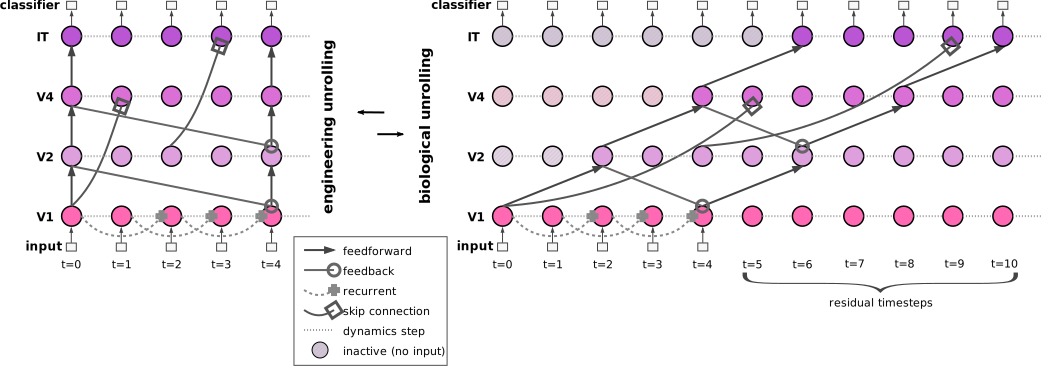
\includegraphics[width=1\linewidth]{rcnn_unrolling_diagram.png}
\end{center}
\caption{\textbf{Network with recurrent, skip, and feedback connections unrolled in engineering versus biological time.} In biological time (\textit{right side}), the network has feedforward connections with delay $\Delta_{FF}=2$, recurrent connections with $\Delta_{RC}=2$, skip connections over two layers with $\Delta_{SK}=5$, and feedback connections over one layer with $\Delta_{FB}=2$. Note that each node has equivalent in- and out- put connections, but only a few are shown here for illustration purposes. By unrolling the network instead in engineering time (\textit{left side}), the delays become $\Delta_{FF}=0$, $\Delta_{RC}=2$, $\Delta_{SK}=1$, $\Delta_{FB}=4$, but the signal flow through the network and time remains identical.} 
\label{fig:time_unrolling}
\end{figure}

\paragraph{Temporally Varied Input Presentation}
For modeling temporal model dynamics the input has to presented over multiple timesteps. The input can be presented as static image over time, combined with a null inputs for certain timesteps, or potentially undergo more complex time-dependent transformations (e.g., by varying the contrast).

The toolbox provides several options to extend static input images over time. By setting the \verb|data_timesteps > 1| config parameter, the dataloaders create an extended view on the data along the time dimension without duplicating the data. This functionality is implemented with the pytorch dataloaders and the ffcv dataloaders. Alternatively, by setting the \verb|data_timesteps = 1| and instead setting the \verb|n_timesteps > 1|, the dataloader load only single input images that are only extend in the forward pass during the model run.

The time extension at runtime can be varied by setting the \verb|data_presentation_pattern| to any boolean string such as \verb|01110|, indicating a temporal sequence of null input (\verb|0|) and input image (\verb|1|). The pattern string is always proportionally stretched or compressed so that its length equals \verb|n_timesteps| and thus each value corresponds to one timestep.
The same functionality is also available by using the time extension with pytorch dataloaders with the option to also realize more complex temporal transformations. 

Overwriting and parameterizing the iterator of the standard pytorch dataloader offers different testing scenarios analogous to common experimental protocols. For example, our `StimulusDuration' loader presents an image after a delay $\delta_i$ for $\delta_s$ duration followed by silent outro period $\delta_o$; the `StimulusInterval' behaves similarly besides also presenting a second identical stimulus with a $\delta_d$ delay after the first; the `StimulusContrast' loader adds to the StimulusDuration setup by multiplying the image input with a scalar to vary its contrast.

% Todo: StimlusNoise

% Todo: Idle Timesteps

\subsection{Network Connectivity}


\subsubsection{Recurrent Connection Types}
% Comment: This subsection details the different recurrence implementations, connecting each to biological evidence and computational considerations. Visual representations should clarify the connectivity patterns.
DynVision contains several options for recurrent connectivity patterns. These options represent different beliefs about the spatial and feature extent of lateral connections. Specifically:

% Paragraph 1: Self-recurrence implementation - Describe within-channel lateral connections, cite Kietzmann et al. 2019 for computational benefits, explain biological motivation from orientation columns (Ohki et al. 2006) and horizontal connections in primary visual cortex.
\paragraph{self-recurrence} connects a unit only to itself. Input is determined by multiplying the feedforward activation tensor with a scalar weight (\cite{Kietzmann2019_21854}, mimicking connections within cortical columns \prettyref{fig:recurrency-types}). 
% Paragraph 2: Full recurrence architecture - Detail dense lateral connectivity, reference Liang & Hu 2015 for original implementation, discuss biological basis in cortical horizontal connections and computational complexity considerations for large-scale models.
\paragraph{full recurrence} applies a standard kernel convolution so that a unit is influenced by a nearby spatial region across all channels, capturing broad lateral connectivity across feature maps. This was introduced by \cite{Liang2015_3367} and is frequently used in the literature (e.g. \cite{Wang2020_117}, \prettyref{fig:recurrency-types}). 
% Paragraph 3: Depthwise and pointwise recurrence - Explain separable convolution approach (Chollet 2017), connection to cortical laminar organization, efficiency benefits over full recurrence demonstrated in mobile architectures, and biological plausibility of channel-wise vs. spatial processing.
\paragraph{depthpointwise recurrence} instead of a full convolution, uses a depthwise (spatial dimension) and then a pointwise (feature dimension) convolution  (see \prettyref{fig:recurrency-types}). This is also known as a depthwise separable convolution and has been used by the computer vision community (\cite{Chollet2017_1800}).While not commonly used in neuroscientific models, it does map onto the structure of lateral recurrence in the visual system observed, for example, in orientation pinwheels and topographic maps. Specifically, visual neurons tend to get input from other neurons that 1.) represent the same spatial location but have different feature preferences (depthwise) and 2.) have the same preferred features but represent different locations in space (pointwise) \citep{Stettler2002_739}.  Depthwise separable convolutions are desirable from an engineering perspective as they reduce the number of parameters compared to a full convolution.
\paragraph{pointdepthwise recurrence} Compared to the depthpointwise recurrence the order of the two partial convolutions is inverted. This follows from the idea that neurons representing similar locations in space are arranged closer together in cortical space so that a signal propagation across features (pointwise) would precede the signal exchange across locations (depthwise) (\prettyref{fig:recurrency-types}). 
% Paragraph 4: Local recurrence innovation - Introduce topographically constrained connectivity inspired by cortical maps (Ohki et al. 2006), cite recent work by Qian et al. 2024 on local connectivity benefits, and connection to retinotopic organization in visual cortex.
\paragraph{local recurrence} aims to capture the 2-D topology of visual cortices. Here, all units in a layer are systematically arranged on a 2-D grid (inspired by cortical organization such as orientation pinwheels in V1 (\cite{Ohki2006_925}, see \prettyref{fig:local-recurrence-mapping}). This mapping requires that the shape information of the input tensor be provided as \verb|dim_y| and \verb|dim_x|. A convolution with kernel size $> 1$ is applied to this grid. The result is that input to each unit is a combination of cortically-local feature and space information (\prettyref{fig:local-recurrence-mapping}. This approach is inspired by LLCNNs \citep{Qian2024_2024.08.06.606687, Bashivan2023_} but also incorporates the spatial retinotopy in the 2-D map. Our approach has similarities to other topographic mappings like All-TNN \citep{Lu2023_} and TDANN \citep{Margalit2023_}, which also map to a combined feature-spatial plane, but have an explicit spatial loss instead of doing a convolution with weight-sharing on this plane. 
This mapping to a 2-D topology requires that the number of channels is a square. If this is not the case, the mapping extends the number of channels to the next square number by duplicating the last channels as with a reflecting boundary. The supplemented channels are removed again in the mapping back to the 3-D tensor.

\paragraph{localdepthwise recurrence} The local recurrence can be extended with an additional depthwise convolution mimicking patchy long-range connections in the visual cortex \citep{Lund1993_148} between units with different feature preferences but the same receptive field.

Standardly, the connectivity matrices $J$ are implemented via kernel convolutions, which reduces the number of parameters to learn (biologically, this corresponds to an assumption that local connectivity statistics are similar for neurons across the cortical sheet). 

% Paragraph 5: Implementation details and performance - Discuss memory requirements, computational complexity scaling, optimization strategies for each recurrence type, and empirical comparisons with baseline architectures from CORnet and other RCNN literature.

%is this right? https://www.cell.com/neuron/fulltext/S0896-6273(02)01029-2

\begin{figure}[ht]
\begin{center}
%\fbox{CCN figure}
\includegraphics[width=.7\linewidth]{recurrency_types.png}
\end{center}
\caption{Four types of kernel convolutions used to effectively realize recurrence: self, full, depthwise, pointwise. For each convolution type, one 3D tensor (Height x Width x Channels) representing a model layer output is shown for two time steps $\Delta t_{rc}$ apart. Each recurrency type uses a specific kind of kernel convolution to add recurrent connections to the layer.} 
\label{fig:recurrency-types}
\end{figure}

\begin{figure}[ht]
\begin{center}
%\fbox{CCN figure}
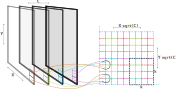
\includegraphics[width=.4\linewidth]{local_recurrence_mapping.png}
\end{center}
\caption{Local recurrence is computed by mapping the 3-D tensor of unit activations onto a 2-D grid so that all features (colors) of one spatial location are arranged close to each other, neighbored by the features of the adjacent spatial locations in a mirrored arrangement. This way, at the borders, the same features at adjacent spatial locations meet and a smooth topographic map can emerge.} 
\label{fig:local-recurrence-mapping}
\end{figure}

%\subsubsection{Implementation as Recurrent Convolutional Module}
% Paragraph 2: implementation details
In our toolbox, the module \verb|RecurrentConnectedConv2d| combines a feedforward 2D convolution (\verb|torch.nn.Conv2d|) operation with a recurrency operation of choice (\verb|recurrence_type|) and handles 
the storage and integration of corresponding hidden states with a variable time delay (\verb|t_recurrence|). The module can extended with a second feedforward convolution by setting a \verb|mid_channels| attributes, as in several popular architectures \citep{Kubilius2018_408385}.

%[TODO: DO WE NEED ALL THIS? -> Move to documentation]The module manages its own hidden state automatically. This can be disabled by setting the size of the hidden state \verb|history_length = 0| and instead passing previous activity tensors as recurrent input manually to the forward call. However, in our model implementations the hidden state of this module is further extended to also provide the stored activations for connections with longer delays by setting \verb|history_length = max(t_feedforward, t_recurrence, t_feedback, t_skip)|.
%Even though we provide the flexible \verb|RecurrentConnectedConv2d| module, its modular structure with interchangeable recurrent types also serves as a template to the user to construct more intricate recurrent layer designs.

\subsubsection{Skip and Feedback Connections}
% Comment: This subsection explains the implementation of long-range connections that enable information flow across layers and time. Emphasis should be on the auto-adaptive feature and biological motivation.

% Paragraph 1: Biological motivation - Connect to cortical feedback pathways from V4 to V1, predictive coding frameworks, attentional modulation mechanisms, and top-down influences on visual processing documented in neuroscience literature.
Besides lateral recurrent connections that link units within one layer across time steps, skip and feedback connections link units across layers and time steps.
Anatomical studies reveal that feedback projections from higher cortical areas like V4 and IT back to V1 are as numerous as feedforward connections, suggesting a fundamental role in visual computation \citep{Felleman1991_1, Salin1995_8234}. 
%[TODO:MOVE ANY OF THESE SPECIFCS TO INTRO]For example, feedback pathways are thought to implement predictive coding mechanisms \citep{Rao1999}, provide context \citep{...}, and attentional modulation \citep{...}.
%Skip connections ...

% Paragraph 2: Feedback/Skip pathway modeling - Explain top-down connections from higher to lower layers, 
Skip and feedback connections describe a similar process: a copy of a layer's output is diverted from the immediate feedforward path to be integrated with to a downstream layer (skip) or an upstream layer (feedback). Thus, we provide a generalized module implementation that covers both cases, and use the same integration strategies as available for the recurrent connection (e.g. additive or multiplicative).
Similar to lateral recurrent connections, the shapes of the source and target layers may not necessarily match, in which case a convolution with a 1x1 kernel is applied to adjust the number of channels, and an up or downsampling operation adjusts the spatial dimensions.

% Paragraph 3: Describe the auto-adaptive signal transformation during first forward pass, eliminating need for manual dimensionality matching across layers, inspired by ResNet innovations but adapted for temporal processing.
To avoid requiring the user to determine the right layer shapes and corresponding transformations in advance, the toolbox offers an \verb|auto_adapt| option, so that the connection can be defined by referencing a source and target layer, and the correct transformation is created upon the first forward pass. This facilitates architecture exploration because connections between layers and orders of operation can easily be swapped without causing errors.

\subsubsection{Integration of (Recurrent) Connections}
Some studies suggest that recurrence may be best modeled as a gain modulation (e.g.\cite{Thorat2022_}). Therefore, in DynVision, the way the recurrent signal is integrated with bottom-up input can be set by \verb|integration_strategy| to either `additive' ($x' = x + h$) or `multiplicative' ($x' = x * (1 + torch.tanh(h))$) or a custom callable function. 
%TODO: find cites that say lateral rec may be gain mod
For test runs the recurrence can be disabled by setting \verb|feedforward_only = True|.

Where the recurrent input is integrated with regards to the convolutions can be selected with the argument \verb|recurrence_target| to either `input', `output', or `middle' (corresponding to prior to any convolutions, between convolution operators, or after all convolutions; see \ref{fig:layer_ordering}). In case there is a mismatch in the spatial dimensions of the recurrent activity tensor with the feedforward activity tensor, an additional up or downsampling is applied via an interpolation or a stride in the convolution operation.

\begin{figure}[ht]
\begin{center}
\includegraphics[width=.8\linewidth]{rctarget_diagram.png}
\end{center}
\caption{\textbf{Illustration recurrent network connectivity in our model and in cortical columns.} \textbf{A)} \textbf{B)} Taken from \citet{Bastos2015_390}.
}
\label{fig:rctarget_diagram}
\end{figure}

\subsubsection{Order of Layer Operations}\label{sec:layer_operations}
The model base classes provide a structure to name and execute the operations of each layer in a flexible order. The activations of each layer are computed by calling its layer operations in the order defined by the \verb|layer_operations| attribute. If a given operation is not defined for a layer, it is skipped.

%The \verb|layer_operations| are defined as a list the modele names either in the config. 
For example, the order of operations used the DyRCNN models presented in this paper is (unless otherwise noted):

\begin{verbatim}
layer_operations: 
    - "rconv"        # apply recurrent convolutional module
    - "addext"       # add external input
    - "addskip"      # add activity from skip connections
    - "addfeedback"  # add activity from feedback connections
    - "tstep"        # apply dynamical systems ode solver step
    - "nonlin"       # apply nonlinearity
    - "delay"        # set and get delayed activations
    - "record"       # record activations in storage buffer
    - "pool"         # apply pooling
\end{verbatim}

The naming of the layers and operations is chosen by the user, except for the reserved operation names: \verb|delay|, which writes the current activity into the hidden states and retrieves a past activity with the correct delay; \verb|tstep|, which accesses the most recent hidden state); and \verb|record|, which stores the current activity in the model's storage buffer.

Any custom model only needs to define its layer names (e.g. \verb|self.layer_names = ['V1', 'V2', 'V4', 'IT'|) and modules in a \verb|_define_architecture()|, following the naming convention \verb|self.<operation>_<layer_name> = <module>|. For layer-unspecific operations, e.g. a non-linearity, the \verb|_<layer_name>| can be omitted.

\subsection{Loss Functions}
The toolbox supports the application of multiple loss functions to be selected in the configs. The default is \verb|loss: ['CrossEntropyLoss', 'EnergyLoss']|. These represent task accuracy and neural activity sparseness as follows:

\paragraph{Category Loss}
Per default we use we use the widely used cross-entropy-loss function as category loss.
The category loss automatically ignores any model output for the residual timesteps, for which model input hasn't yet reached the classifier. Additionally, there is a \verb|loss_reaction_time| setting that further removes the initial $n$ timesteps (after any residual timesteps) from consideration for the category loss as desired.

\paragraph{Energy Loss}
Activity regularization promotes more stable network activity and is biologically motivated by mechanisms of homeostatic plasticity \cite{Keck2017_20160158}. In the toolbox, we add an effective activity regularization via an energy loss function \citep[inspired by][]{Butkus2024_} that penalizes large unit responses, thus mimicking the metabolic constraints of spike generation in the brain.
This loss function accesses the activations of any convolutional or linear module from the computational graph without the need for any additional storing of activation tensors. The energy loss is defined as the p-norm (default is $p=1$) of the activation tensor $r_m$ of module $m$ divided by its number of units $N_m$ and averaged across all modules $M$ (\prettyref{eq:energy_loss}).

\begin{equation}
\label{eq:energy_loss}
\mathcal{L}_{energy} = \frac{1}{M}\sum_{m=1}^M\left(\frac{1}{N_m}\sum_{n=1}^{N_m} |r_{m,n}|^{p} \right)^{\frac{1}{p}}
\end{equation}

Adding a weight decay further adds weight regularization to promotes network stability and more efficient and sparse coding, further modeling metabolic constraints.

Any loss function-specific configurations are set in the confis as dicts with \verb|loss_config: [<loss_name>: <loss_configs>]|. A weighting of the individual loss contributions is coordinated with a \verb|weight| scalar value in the loss configs.
The available loss functions can be extended by adding a corresponding implementation or wrapper class for a pytorch loss function to the 'dynvision/losses/' folder. The BaseLoss parent class provides consistent input processing, shape validation, and reduction over the batch and time dimension.

\subsection{Additional Biological Components}
% Comment: This subsection covers supporting components that enhance biological realism. Each component should be motivated by neural evidence and implementation details provided.

% Paragraph 1: Supralinear activation functions - Reference Rubin et al. 2015 work on stabilized supralinear networks, explain implementation of divisive normalization and biological basis in dendritic integration, connection to cortical response properties.
\paragraph{Supralinearity}
Individual neurons often exhibit nonlinear amplification, where strong inputs lead to disproportionately large activations. The influence of recurrence is necessary to stabilize this explosive activity \citep{Sanzeni2020_e54875}. The toolbox allows users to apply a supralinear activation function inspired by models of visual cortex \cite{Rubin2015_402, Lindsay2019_} to encourage networks to make effective use of recurrent connections for regularizing feedforward activity. 

% Paragraph 2: Retina-inspired preprocessing - Detail preprocessing components that model early visual processing, center-surround organization, contrast adaptation, and their implementation in the DynVision framework.
\paragraph{Input Preprocessing}
Having a dedicated input layer to preprocess the input stimuli is a common component of vision models. The toolbox includes two biologically inspired versions of this: 1.) a simple adaption factor (fixed or learnable) that reduces the input values to the network over time so that it is necessarily more dependent on recurrent connections to retain information, 2.) a layer representing the retina and LGN and their representational bottleneck, as described in \cite{Lindsey2019_}.

\subsection{Reference Models}
To facilitate rapid experimentation and benchmarking, the toolbox integrates implementations of several well-established neural network architectures from the literature, including AlexNet \citep{Krizhevsky2012_}, the ResNet family \citep{He2016_770}, CORNet-RT \citep{Schrimpf2020_407007}, and CordsNet \citep{Soo2024_}. In addition to these models, users can easily instantiate the showcase models introduced in this paper, such as DyRCNNx2, DyRCNNx4, DyRCNNx8. The framework also supports the automatic loading of pre-trained weights, with mechanisms in-place to correctly match parameters even when model configurations have been modified (e.g., additional layers or biologically inspired features added). Notably, models are designed to be data context-aware, meaning they are automatically initialized with the appropriate number of output classes based on the provided dataset. The toolbox further enables selective training of only non-pre-trained parameters or full model fine-tuning, offering flexibility for transfer learning applications.

\subsection{Software Design}
% Comment: This subsection explains the software engineering approach that enables the biological modeling. The description should emphasize how good software design supports scientific goals.
DynVision is designed with scientific exploration in mind. We follow best principles for scientific software engineering to make the toolbox transparent and easy to use. 

\paragraph{Modularity}
% Paragraph 2: Modularity principle - Explain how modular design enables systematic experimentation by allowing researchers to vary specific components (recurrence type, time constants, connectivity) while controlling others, inspired by CORnet's success in Brain-Score optimization through systematic architecture exploration.
The fundamental advantage of using modeling approaches in neuroscience is that contrary to actual brains models allow for precise control and monitoring of each and every variable and therefore make it possible to probe their respective influence on model behavior. Such probing investigations may take the form of parameter sweeps, changing the order of operations, adding/removing/replacing individual operations, and inserting targeted perturbations. In order to effectively explore these options, the modeling environment must make the interfaces to the variables of interest explicit and make the components interoperable so that the model runs seamlessly in each configuration.
The DynVision toolbox employs this paradigm of modularity by constructing core model and training capabilities by combining specialized base classes via multiple inheritance, defining the model's architecture as a sequence of layers, and each layer as a sequence of operations. This two-tier organization allows for flexible arrangement of computational components. Layer operations are built from interchangeable components including recurrence types,  connectivity patterns, dynamics solvers, and signal delays which can be reordered and swapped without changing the overall model handling. This modularity enables researchers to conduct controlled experiments where specific components are varied while others are held constant, facilitating systematic exploration of the design space.

\paragraph{Configuration-driven Modeling}
% Paragraph 3: Configuration-driven approach - Detail how YAML-based configuration separates scientific modeling decisions from implementation details, enabling reproducible parameter space exploration and systematic comparison of architectural choices, addressing limitations identified in current RCNN literature.
Our toolbox aims to separate the many scientific modeling decisions from the technical implementation details as well as possible by designing a code framework that is generalized and flexible enough to allow for many variations while remaining computationally efficient. In support of this, model configuration choices are defined in a YAML-based config schema which is integrated into the workflow via a rigorous parameter handling pipeline. The advantages are i) a lower coding barrier for developing and testing complex but efficient models, ii) reproducibilty, reusability, and systematic parameter space space exploration, iii) making architectural choices, like the order of layer operation or type of time-unrolling, explicit and visible, iv) integrating technical advances independent from a model design.

\paragraph{Interoperability}
% Paragraph 4: Integration philosophy - Explain integration with established ML tools (PyTorch Lightning for training, Snakemake for workflows) rather than creating isolated framework, learning from successful adoption patterns in CORnet and other neuroscience-inspired models.
To better integrate technical advances, the toolbox relies on: PyTorch \citep{Paszke2017_} for performative tensor operations and machine learning utilities; PyTorch lightning \citep{Falcon2020_} to seamlessly organize state-of-the-art training, validation, and testing procedures and allocate them on GPU or CPU resources; ffcv dataloader \citep{Leclerc2023_12011} to optimize the computational bottleneck of data loading and transfer; the snakemake workflow manager \citep{Molder2021_33} to facilitate automatization, scalability, and portability of workflows; yaml config scripts and Pydantic\footnote{\url{https://docs.pydantic.dev/latest/}} parameter handling to provide a high-level, human-readable interface; and a cookiecutter-based structure to aid with a clear folder organization. This strong reliance on existing tools and developer communities aids in maintainability and further promotes well-defined interfaces for adding new components, models, optimization, and analysis methods

\subsubsection{Base Classes}
% Comment: This subsection explains the organization of core model functionalities implemented in five specialized base classes that are combined via multiple inheritance in the main BaseModel class.
DynVision employs a modular base class architecture that separates concerns into specialized components, each addressing distinct aspects of neural network modeling. This design leverages multiple inheritance and mixin classes to achieve both flexibility and maintainability. A \verb|BaseModel| class integrates all the components while researchers can also compose models with a subset of base classes or add additional parent classes with a specific functionality while ensuring consistent interfaces across the toolbox.

% Paragraph 1: TempralBase - Explain the handling of temporal dynamics and the forward pass architecture
\paragraph{TemporalBase}
The \verb|TempralBase| class robustly handles the processing of temporally extended input. It implements the utility to effectively manage the time dimension of signal tensors (\verb|[batch_size, n_timesteps, n_channels, dim_y, dim_x]|), including temporal unrolling, and residual timesteps. The \verb|forward()| function processes the input sequentially across time, where at each timestep, the \verb|_forward()| function executes layer-specific operations in a configurable order (see \prettyref{sec:layer_operations}).

% Paragraph 2: LightningBase - PyTorch Lightning integration benefits for neuroscience research
\paragraph{LightningBase}
The \verb|LightningBase| class integrates PyTorch Lightning to address much of the engineering overhead in training models in PyTorch, including automatic mixed-precision training, automatic logging, checkpointing, and hardware acceleration across single GPUs to multi-node clusters, and hyperparameter optimization utilites. This class specifically provides further abstraction by implementing a Lightning model tailored for training recurrent convolutional networks with all relevant configuration parameters set to reasonable defaults and editable the human-readable config files.

% Paragraph 3: StorageBuffer - Memory-efficient analysis of temporal neural responses
\paragraph{StorageBuffer}
The \verb|StorageBuffer| component addresses the unique memory requirements of storing model output, activations, and hidden states across timesteps. It selectively records the model in- and out- puts and layer activations in training, validation, and testing context with fixed or cyclic recording strategies, variable buffer sizes, and optional CPU offloading strategies to capture population dynamics without exhausting GPU memory. This capability is crucial for comparing model responses against electrophysiological recordings, as it preserves the full temporal evolution of neural activations across the model over extended stimulus presentations. Further, the class implements utility functions for managing and exporting the recordings as tensor, dict, or pandas.DataFrame that combines labels, predictions, batch and sample indices, timesteps, and classifier unit activations.

% Paragraph 4: DtypeDeviceCoordinator - Precision management for biological parameters
\paragraph{DtypeDeviceCoordinator}
While most of the device and dtype coordination is already handled efficiently by PyTorch Lightning, the \verb|DtypeDeviceCoordinator| system further ensures dtype and device consistency across child and parent class (that may not be derived from a LightningModule), variables in storage buffers, and between dataloader and model trainer.

% Paragraph 5: Monitoring - Systematic debugging and analysis for complex biological models
\paragraph{Monitoring}
The \verb|Monitoring| class provides structured logging and debugging of the model, training, and system parameters, including detailed memory usage, including automatic detection of common numerical issues (NaN gradients, parameter drift), systematic tracking of parameter evolution, and real-time visualization of network dynamics and weight distributions. The logging capabilities integrate with the Lightning logging mechanism and its interface to external monitoring tools such as Weights\&Biases \footnote{\url{https://wandb.ai}}.

\subsubsection{Parameter Handling}
% Comment: Parameter management framework - Describe the hierarchical parameter system with validation, type checking, and configuration inheritance, parameter expansion enabling systematic exploration of biological parameter spaces.

% Paragraph 1: Separating code and configuration with human-readable config files that are hierachically organized
\paragraph{Hierarchical Configuration}
The toolbox implements a comprehensive parameter management framework that separates configuration from code implementation, enhancing reproducibility and systematic exploration of biological parameter spaces. The system employs human-readable YAML configuration files organized hierarchically across specialized domains: \texttt{config\_defaults.yaml} establishes baseline model parameters and system settings, \texttt{config\_data.yaml} defines dataset specifications \texttt{config\_experiments.yaml} specifies data selection and parameter sweeps protocols for model testing scenarios.
The \texttt{config\_workflow.yaml} file sits at the top of the hierarchy and defines any parameters that are relevant for the current application overwriting duplicate default settings in other config files. Further, \texttt{config\_modes.yaml} provide whole parameter presets to rapidly switch between configuration contexts such as  (\texttt{local} for local test runs, \texttt{debug} for verbose logging, \texttt{large\_dataset} for memory-optimized processing, and \texttt{distributed} for multi-device cluster execution.
This hierarchical organization enables researchers to override specific parameters at appropriate abstraction levels while maintaining consistent defaults.

\paragraph{Parameter Expansions and Overwrites}
% Paragraph 2: Extension of configs in snakemake by optional overwrites via command-line arguments and expanding over lists of parameter values. Final runtime configs are stored for reproducibility. Relevant config values are passed to scripts in snakemake rules.
The Snakemake workflow system extends this configuration framework through dynamic parameter expansion and command-line integration. Configuration parameters can be selectively overridden via command-line arguments (\texttt{snakemake --config model\_name=DyRCNNx4 lr=0.001}), enabling rapid prototyping without modifying configuration files. Parameter lists are automatically expanded into Cartesian products for systematic exploration (\texttt{recurrence\_type: [full, self, depthwise]} generates separate jobs for each architecture variant), while runtime configurations are automatically archived alongside experimental outputs to ensure complete reproducibility. 

\paragraph{Parameter Parsing}
% Paragraph 3: Parsing, alias evaluation, validation, and param utilities of script arguments via dedicated pydantic classes (ModelParams, DataParams, TrainerParams and their composite classes InitParams, TrainingParams, TestingParams)
The script-level parameter handling employs type-safe Pydantic classes that provide robust validation, automatic type conversion, and biological constraint checking. Specialized parameter classes (\texttt{ModelParams}, \texttt{DataParams}, \texttt{TrainerParams}) encapsulate domain-specific validation logic and computed properties, while composite classes (\texttt{InitParams}, \texttt{TrainingParams}, \texttt{TestingParams}) combine these components for script-specific processing. The system supports flexible parameter aliasing (\texttt{lr} $\rightarrow$ \texttt{learning\_rate}, \texttt{rctype} $\rightarrow$ \texttt{recurrence\_type}) and implements context-aware validation that enforces system and biological feasibility constraints and cross-parameter consistency checks, e.g., time delays are integer multiples of time resolution, or batch size and learning rate scaling for multi-device training and gradient accumulation.

\subsubsection{Data Handling}
The toolbox addresses data management challenges in a configuration-driven pipeline that supports the computational demands of temporal modeling while maintaining experimental flexibility.

% Described organization of raw data into training, validation, and testing datasets and subsets without storage overhead via symlink collections
The toolbox implements a symbolic link-based organization system in the snakemake workflow scripts that eliminates storage redundancy while enabling flexible experimental configurations. Raw datasets are automatically partitioned into training, and testing subsets.

% Describe automatic dataset grouping into subset by defining a corresponding list of class indices in config_data.yaml. The input files are symlinked into a corresponding folder and the label indices are transformed to be consistent with the full dataset with all classes the model was trained on.
Data subsets can be further subsampled into groups containing only a selection of classes defined by specifying the class indices in \verb|config_data.yaml|. The system automatically handles label index transformations to maintain consistency with the full dataset, ensuring that models trained on complete datasets can be seamlessly evaluated on class subsets. Besides making testing faster, this functionality is particularly to vary the testing difficulty or investigate category-specific neural responses.

% Describe that finetuning on a new dataset is made convenient by automatically adapting the classifying layer to the number of classes in a the given dataset
For model training, the architecture is validated to be consistent with the training dataset and automatically adapts the classifier layers to the number of presented classes. This streamlines transfer learning and fine-tuning models on different datasets.

% adding a new dataset: data statistics for normalization, transforms, data resolutions defined in config_data.yaml. if data is available in torchvision it is downloaded, or it is to be placed in the data/raw folder. (add lookup class name list) 
 

% Describe fast data loading with FFCV achieving speedup over standard PyTorch dataloaders, preprocessing optimization, and resulting performance improvements for temporal modeling.
Recognizing that temporal neural network models require processing sequences of images over many timesteps, the toolbox integrates FFCV (Fast Forward Computer Vision) \citep{Leclerc2023_12011} data loading, achieving speedup compared to standard PyTorch DataLoaders. The accelerated preprocessing pipeline includes GPU-optimized transformations (incl. expanding for expanding timesteps) and direct memory mapping, reducing CPU-GPU transfer overhead that would otherwise dominate training time for models requiring hundreds of temporal integration steps.

\subsubsection{Workflow Management}
% Comment: This subsection demonstrates how the toolbox integrates the components in the model development and evaluation lifecylce into workflows. The emphasis should be on reproducibility and scalability.
%Snakemake integration benefits - Explain how the rule-based workflow management of snakemake enables reproducible experiments, dependency tracking, and automatic parallelization, addressing reproducibility challenges in computational neuroscience research.
The toolbox employs Snakemake-based \citep{Molder2021_33} workflow orchestration to integrate the complete model development and evaluation lifecycle into reproducible, scalable computational pipelines. The rule-based dependency system automatically manages the sequential stages from raw data acquisition through dataset organization, model initialization, training, analysis, and visualization ensuring that each computational step executes only when its prerequisites are satisfied and input data has changed. This approach addresses critical reproducibility challenges by maintaining explicit dependency tracking, assigning parameter selections to specific steps, enabling automatic parallelization of independent tasks, and providing deterministic execution paths that can be precisely replicated across different computing environments. 

%Scalability and Portability support - Explain scaling from laptops to HPC systems, resource management for memory-intensive temporal models, flexible centralized path management, and distributed training capabilities for large-scale experiments.
The workflow architecture seamlessly scales from individual laptops to high-performance computing clusters through adaptive resource management and centralized path configuration, accommodating the substantial memory and computational demands of biologically plausible temporal models that require extended simulation periods with fine-grained timesteps and substantial hidden state storage.

% \begin{table}[ht]
% \centering
% \caption{\textbf{Comparison of DynVision with biologically plausible neural network frameworks.} Feature comparison across different approaches to biologically inspired vision models shows DynVision's unique position combining continuous dynamics, systematic exploration capabilities, and modern ML infrastructure.}
% \begin{tabular}{lcccccc}
% \hline
% \textbf{Feature} & \textbf{DynVision} & \textbf{CORnet} & \textbf{VOneNet} & \textbf{ORGaNICs} & \textbf{Neural ODEs} & \textbf{BLT/Spike-driven} \\
% \hline
% Continuous dynamics & \checkmark & \texttimes & \texttimes & \checkmark & \checkmark & \checkmark \\
% Heterogeneous delays & \checkmark & \texttimes & \texttimes & \texttimes & \texttimes & \checkmark \\
% Multiple recurrence types & \checkmark & Limited & \texttimes & \texttimes & \texttimes & Limited \\
% Vision-optimized & \checkmark & \checkmark & \checkmark & \texttimes & \texttimes & \checkmark \\
% Workflow management & \checkmark & \texttimes & \texttimes & \texttimes & \texttimes & \texttimes \\
% Biological constraints & \checkmark & \checkmark & \checkmark & \checkmark & Limited & \checkmark \\
% Systematic exploration & \checkmark & \texttimes & \texttimes & \texttimes & \texttimes & \texttimes \\
% Performance optimization & \checkmark & \checkmark & \checkmark & \texttimes & \checkmark & \checkmark \\
% Brain-Score validation & \checkmark & \checkmark & \checkmark & \texttimes & \texttimes & Limited \\
% \hline
% \end{tabular}
% \label{tab:framework_comparison}
% \end{table}

% \subsection{Performance Optimizations}
% % Comment: This subsection addresses practical concerns about computational efficiency. The message should be that biological plausibility doesn't require sacrificing performance.

% % Paragraph 1: Mixed precision training support - Explain implementation of float16/bfloat16 computation, memory savings for temporal sequences, and accuracy considerations for biological parameters with different numerical ranges.
% lightning optimizations
% % Paragraph 2: Memory management strategies - Detail response storage optimization, activation checkpointing for long sequences, and GPU memory utilization strategies inspired by Neural ODEs' memory-efficient implementations.
% data buffer memory scaling with different strategies

% % Paragraph 3: FFCV dataloader integration - Present benchmarking results showing 52% speedup over standard PyTorch dataloaders, explain preprocessing optimization and bottleneck elimination for temporal data.
% pytorch for initialization and testing, ffcv (optionally) for training.

% % Paragraph 4: Recurrent operation optimization - Describe computational costs of different recurrence types, memory layout optimization, and kernel fusion strategies for GPU acceleration.

% % Paragraph 5: Scaling performance - Discuss single-GPU to multi-GPU scaling, distributed training considerations for temporal models, and cluster utilization efficiency for large-scale experiments.
% efficient multi-gpu scaling (nearly scales with number of devices)



\section{Demonstrations and Results}
% Comment: This section demonstrates DynVision's capabilities through concrete examples and benchmarks. The demonstrations should showcase both technical performance and novel scientific insights enabled by the toolbox.
We built this toolbox to generalize biological RCNN network models and make them flexibly editable for systematic exploration. To demonstrate its capabilities, we focus on our primary working model, the DyRCNNx8, inspired by existing architectures in the literature. We systematically explore the modeling parameter space to identify optimal configurations, then validate the biological plausibility of the resulting models by comparing against neural data and behavioral observations. Having established that our DyRCNN models exhibit biologically realistic dynamics, we demonstrate the framework's generality by showing it can precisely recreate established models from the literature (CORnet-RT and CordsNet). Finally, we provide comprehensive computational benchmarking showing that the toolbox delivers significant performance advantages, and detail how specific modeling choices affect training speed, GPU memory usage, and model complexity.

\subsection{Model Architecture}
\label{model_details}
The version of the DyRCNNx8 model analyzed throughout this section contains variants of lateral recurrence and skip connections. Impacts of feedback connections will be explored in future work.

The architecture and order of operations is defined as follows:

\begin{itemize}
    \item[\textbf{[V1]}] \textbf{Conv2d}(\textit{in=3, out=64, k=5×5, s=2}) \textbf{→ ReLU → Conv2d}(\textit{in=64, out=64, k=5×5, s=1}) \textbf{→ +Recurrence} (\textit{$\Delta_{RC}=6ms$}) \textbf{→ Euler Step} (\textit{$dt=2ms$, $\tau=9ms$}) \textbf{→ ReLU → Delay} (\textit{$\Delta_{FF}=0ms$}) \textbf{→ MaxPool}(\textit{3×3, s=2})
    
    \item[\textbf{[V2]}] \textbf{Conv2d}(\textit{in=64, out=144, k=3×3, s=2}) \textbf{→ ReLU → Conv2d}(\textit{in=144, out=144, k=3×3, s=1}) \textbf{→ +Recurrence} (\textit{$\Delta_{RC}=6ms$}) \textbf{→ Euler Step} (\textit{$dt=2ms$, $\tau=9ms$}) \textbf{→ ReLU → Delay} (\textit{$\Delta_{FF}=0ms$}) \textbf{→ MaxPool}(\textit{3×3, s=2})
    
    \item[\textbf{[V4]}] \textbf{Conv2d}(\textit{in=144, out=256, k=3×3, s=2}) \textbf{→ ReLU → Conv2d}(\textit{in=256, out=256, k=3×3, s=1}) \textbf{→ +Recurrence} (\textit{$\Delta_{RC}=6ms$}) \textbf{→ +Skip}(\textit{V1, $\Delta_{SK}=0ms$}) \textbf{→ Euler Step} (\textit{$dt=2ms$, $\tau=9ms$}) \textbf{→ ReLU → Delay} (\textit{$\Delta_{FF}=0ms$})
    
    \item[\textbf{[IT]}] \textbf{Conv2d}(\textit{in=256, out=529, k=3×3, s=2}) \textbf{→ ReLU → Conv2d}(\textit{in=529, out=529, k=3×3, s=1}) \textbf{→ +Recurrence} (\textit{$\Delta_{RC}=6ms$}) \textbf{→ +Skip}(\textit{V2, $\Delta_{SK}=0ms$}) \textbf{→ Euler Step} (\textit{$dt=2ms$, $\tau=9ms$}) \textbf{→ ReLU → Delay} (\textit{$\Delta_{FF}=0ms$})
    
    \item[\textbf{[Classifier]}] \textbf{AdaptiveAvgPool2d}(\textit{1}) \textbf{→ Flatten → Linear}(\textit{529 → 10})
    
\end{itemize}

Further parameters and training details can be seen in Table \ref{param_table}.

\begin{table} %[htbp]
\centering
\caption{Default Training Configuration}
\label{tab:training_config}
\begin{tabular}{lll}
\toprule
\textbf{Parameter} & \textbf{Value} & \textbf{Description} \\
\midrule
\multicolumn{3}{l}{\textbf{Temporal Dynamics}} \\
Time steps & 20 & Number of simulation timesteps \\
Resolution ($dt$) & 2 ms & Integration time step \\
Time constant ($\tau$) & 5 ms & Neural time constant \\
Feedforward delay ($\Delta_{FF}$) & 30 ms & Feedforward connection delay \\
Skip connection delay ($\Delta_{SK}$) & 0 ms & Skip connection delay \\
Recurrent delay ($\Delta_{RC}$) & 6 ms & Recurrent connection delay \\
Integration strategy & Additive & Activity integration method \\
Dynamics solver & Euler & Numerical ODE solver \\
Recurrence target & Output & Recurrence applied to layer output \\
\midrule
\multicolumn{3}{l}{\textbf{Architecture Configuration}} \\
Skip connections & Enabled & V1→V4, V2→IT \\
Feedback connections & Disabled & No top-down connections \\
Normalization & None & No BatchNorm/LayerNorm \\
\midrule
\multicolumn{3}{l}{\textbf{Training Setup}} \\
Training epochs & 200 & Total training duration \\
Datasets & ImageNette & 224px, 10 classes \\
Batch size & 256 & Training batch size \\
Initial learning rate & 0.0008 & Base learning rate \\
LR scheduler & CosineAnnealingLR & $T_{max}=250$ \\
Recurrent LR factor & 0.2 & LR scaling for recurrent weights \\
Optimizer & Adam & Optimization algorithm \\
Weight decay & 0.0005 & L2 regularization \\
\midrule
\multicolumn{3}{l}{\textbf{Weight Initialization}} \\
Feedforward weights & Truncated Normal & mean=0.0, std=0.004 \\
Recurrent weights & Uniform & range=[-0.001, 0] \\
Bias initialization & Zero & All biases set to 0 \\
\midrule
\multicolumn{3}{l}{\textbf{Loss Function}} \\
Primary loss & Cross-entropy & Classification loss \\
Auxiliary loss & Energy loss (0.2×) & Biological constraint \\  % ToDo: update
Loss reaction time & 4 ms & No temporal offset for loss \\
\midrule
\multicolumn{3}{l}{\textbf{Optimization}} \\
Gradient accumulation & 4 batches & Effective batch size: 1024 \\
Precision & bf16-mixed & Mixed precision training \\
Gradient clipping & Norm, value=1.0 & Gradient norm clipping \\
\bottomrule
\end{tabular}
\label{param_table}
\end{table}


\subsection{Model Training}
\label{sec:model_training}

\subsubsection{Energy Loss and Temporal PPresentation Pattern}
A critical consideration when training biologically plausible recurrent networks is balancing task performance with biological constraints. The energy loss function (Eq. \ref{eq:energy_loss}) implements a metabolic constraint that promotes sparse, efficient neural coding. However, the relative weighting between the cross-entropy classification loss and the energy regularization loss affects both training dynamics and the final network behavior.

To establish appropriate training parameters for subsequent experiments, we systematically explored different energy loss weights during training. Figure \ref{fig:energyloss_training} shows training and validation accuracy curves, the evolution of loss components, and most importantly, the temporal dynamics of network activity at different stages of training (early, middle, and late epochs).

These results demonstrate that [DESCRIBE KEY FINDINGS - e.g., optimal energy loss weight balances accuracy and biological plausibility, dynamics evolve from unstable early training to stable late training, choice of weight affects final temporal response patterns]. Based on these findings, we selected an energy loss weight of 0.4 and trained models for 300 epochs for all subsequent analyses, ensuring stable dynamics while maintaining high classification performance.

% TODO: Add actual figure when available
\begin{figure}[ht]
    \begin{center}
    \includegraphics[width=\linewidth]{training_energyloss_pattern=1.png}
    \end{center}
    \caption{\textbf{Training DyRCNNx8 model with different energy loss weights.}
    \textit{A)} Training and validation accuracy across 200 epochs for different energy loss weights (0.0, 0.1, 0.2, 0.5, 1.0).
    \textit{B)} Evolution of cross-entropy and energy loss components during training.
    \textit{C)} Temporal dynamics of layer activations at epoch 20 (early training), epoch 100 (mid-training), and epoch 200 (late training), showing the evolution from unstable to stable response patterns.
    \textit{D)} Final test accuracy and mean energy consumption for each weight setting, demonstrating the trade-off between task performance and biological constraint satisfaction.
    }
\label{fig:energyloss_training}
\end{figure}
\begin{figure}[ht]
    \begin{center}
    \includegraphics[width=\linewidth]{training_energyloss_pattern=1011.png}
    \end{center}
    \caption{\textbf{Training DyRCNNx8 model with different energy loss weights.}
    \textit{A)} Training and validation accuracy across 200 epochs for different energy loss weights (0.0, 0.1, 0.2, 0.5, 1.0).
    \textit{B)} Evolution of cross-entropy and energy loss components during training.
    \textit{C)} Temporal dynamics of layer activations at epoch 20 (early training), epoch 100 (mid-training), and epoch 200 (late training), showing the evolution from unstable to stable response patterns.
    \textit{D)} Final test accuracy and mean energy consumption for each weight setting, demonstrating the trade-off between task performance and biological constraint satisfaction.
    }
\label{fig:energyloss_training}
\end{figure}

With these training parameters established, we built and trained DyRCNNx8 models with each of our six main forms of lateral recurrence available (self, full, depthpointwise, pointdepthwise, local, and localdepthwise).

As can be seen in Figure \ref{fig:rctype_training}, models with all forms of recurrence are able to train to high accuracy and show stable output dynamics. The model with \textbf{full} recurrence has the most parameters and also highest performance by a small margin.

\begin{figure}[ht]
\begin{center}
\includegraphics[width=\linewidth]{training.png}
\end{center}
\caption{\textbf{Training the DyRCNNx8 model with different recurrence types.}
All models were trained with 20 timesteps, $dt=2$, $\tau=9$, $\Delta_{FF}=0$, $\Delta_{RC}=6$, skip connections, and energy loss weight of 0.2 on imagenette for 200 epochs.
\textit{A)} Training (solid) and validation (dotted) accuracy for the model versions with different recurrence types. \textit{B)} The model was trained with a combined loss: cross-entropy loss measuring classification performance and energy loss measuring mean unit activations. \textit{C)} Testing the accuracy of the models on 50 timesteps with input presentation for the first 30 timesteps. Dashed lines show the confidence, the softmax value of the target classifier unit. Values are for 256 randomly chosen images. \textit{D)} Comparison of the models' number of parameters, training speed, and performance.
% DyRCNNx8:tsteps=20+rctype=*+dt=2+tau=9+tff=0+trc=6+skip=true_0019_imagenette_trained_all
}
\label{fig:rctype_training}
\end{figure}

\subsubsection{Equivalence of Engineering and Biological Time Unrolling}
A unique feature of DynVision is the ability to train networks using either engineering time (where $\Delta_{FF}=0$) or biological time (where $\Delta_{FF}>0$) unrolling. As described in Section 2.2, these two approaches should produce mathematically equivalent dynamics when delays are properly adjusted. We validate this theoretical prediction empirically by training a model in engineering time and testing it in both engineering and biological time configurations.

\begin{figure}[ht]
    \begin{center}
        \includegraphics[width=.4\linewidth]{unrolling.png}
    \end{center}
    % DyRCNNx8:tsteps=40+rctype=full+dt=2+tau=9+tff=*+skip=true+feedback=true_0030_imagenette_trained_StimulusDuration:dsteps=70+intro=0+stim=35_one
    \caption{\textbf{Equivalence of engineering and biological time unrolling.} This DyRCNNx8 model was trained with full recurrence, skip (V1$\rightarrow$V4; V2$\rightarrow$IT), and feedback connections (IT$\rightarrow$V2; V4$\rightarrow$V1) on input with 40 timesteps unrolled in engineering time ($\Delta_{FF}=0$~ms, $\Delta_{SK}=0$~ms, $\Delta_{FB}=34$~ms, $\Delta_{RC}=6$~ms, $\tau=9$~ms, $dt=2$~ms), and then tested in both engineering time and biological time ($\Delta_{FF}=10$~ms, $\Delta_{SK}=20$~ms, $\Delta_{FB}=14$~ms, rest identical) on a single image presented for 35 timesteps followed by 35 timesteps of null input (indicated by the grey step function). Each configuration yields equivalent model responses, validating the mathematical framework and demonstrating computational flexibility.}
    \label{fig:unrolling_equivalence}
\end{figure}

As shown in Figure \ref{fig:unrolling_equivalence}, the model produces identical temporal dynamics regardless of the unrolling scheme, confirming that researchers can choose the computationally more efficient engineering time for training while maintaining the ability to interpret results in biological time. This flexibility is particularly valuable when comparing model predictions to neural recordings where real-world propagation delays matter.


\subsection{Evaluation of Modeling Choices}
\label{sec:modeling_choices}
A main motivation for providing this toolbox is our belief that the research community needs to explore the space of RCNNs more thoroughly in order to understand the impact of different parameter regimes on model properties. Here, we systematically examine how specific modeling choices affect learned dynamics, ultimately justifying the parameter selections used for our DyRCNN models in subsequent biological validation experiments.


\subsubsection{Loss Reaction Time}
The evaluation of the training loss can be restricted to a subset of timesteps. The exact number and placement of these timesteps varies across studies, including models that use all timesteps \citep{Spoerer2020_e1008215}, the last timestep \citep{Kubilius2018_408385}, or a number of timesteps in between \citep{Soo2024_}. It is therefore important to understand the impacts of this parameter choice.

In \prettyref{fig:lossrt}, we show dynamics across layers when different timespans of the output are used for the loss function. These choices have clear qualitative impacts on dynamics, particularly at later layers. When the entire output time is used for the loss ($lossrt=0$), activity ramps up quickly and then settles into a lower stable state. Using only a small number of timepoints at the end of stimulus presentation ($lossrt=98$) leads to unstable dynamics. Therefore, we can see that while using fewer timesteps reduces computational costs, it also reduces stability and biological plausibility. Note: these results are based on the DyRCNNx4 model.

% TODO: Add figure for loss reaction time analysis
The results suggest that it is helpful to compute the loss for most of the timesteps in order to promote stability and realistic dynamics. This is further motivated biologially as object classification in biological time is an continously ongoing task that is usually not limited to a certain timespan within the object presentation. \citet{Spoerer2020_e1008215} further argue that using all timesteps encourages the model to achieve a correct classification as quickly as possible and therefore produce better interpretabile reaction times.
However, we also see that this incentive to classify quickly, when overtrained, can lead to strong overshoot and oscillatory activity that can make the model response more unstable when presented with temporally different inputs.
Therefore, we find a small loss reaction time that excludes only the first few timesteps after image presentation (in engineering time) to be a well balanced modelling choice.


\subsubsection{Initial Idle Period during Training}
Initializing hidden states in recurrent models is realized in various ways. CorNet initializes hidden states with zeros, whereas the hidden states of our DyRCNN model produce None (i.e. no recurrent signal integration) when they are not yet populated. CordsNet addresses this issue with preceeding its forward pass with a number of idle timesteps, where only a null input is provided, to allow self-generated activity to stabilize and populate the hidden states. We systematically tested whether this design choice benefits our DyRCNN architecture.
As null input we choose for the idle timeteps we choose zero tensors representing a neutral contrast-free input, which corresponds to the average pixel value, since the input images are normalized.

\begin{figure}[ht]
\begin{center}
\includegraphics[width=\linewidth]{timesteps_response_tripytch.png}
\end{center}
\caption{\textbf{Effect of initial idle timesteps on training dynamics.} [TODO: Add detailed caption describing comparison of models trained with and without idle periods, showing no benefit for DyRCNN architecture due to energy loss regularization.]}
\label{fig:timesteps_tripytch}
\end{figure}

As shown in Figure \ref{fig:timesteps_tripytch}, for our model there is no benefit for training with initial idle timesteps. This is likely because the energy loss regularization provides sufficient constraint on activity levels from the start of training, eliminating the need for an idle stabilization period. This simplifies the training protocol while maintaining stable dynamics.

\subsubsection{Target of Recurrent Connections}
Where exactly the recurrent input is incorporated into the feedforward computations is a modeling choice that usually does not receive much explicit attention. Yet, we show here that different choices can lead to qualitatively different dynamics.

In Figure \ref{fig:connection_tripytch}, activity dynamics across layers are shown for recurrence fed into the input, middle, and output of a layer. The `input' setting integrates the recurrent activations with the feedforward activations before they are fed into the convolution(s), the `output' setting integrates the activations after the convolution(s), and if a \verb|mid_channel| value is provided and there are two convolutions in a layer, the 'middle' setting integrates the recurrence in between the convolutions. In case of `output' and `middle' targets, the recurrent activation tensor is upsampled along the spatial dimensions, using a nearest neighbors algorithm, to compensate for the change in tensor shape due to the strides of the convolutions. Feeding recurrent inputs into the output of the layer's computations leads to particularly distinct dynamics. This highlights the need for tools that allow us to thoroughly explore the parameter space of RCNNs for the purposes of biological modeling.

\begin{figure}[ht]
\begin{center}
\includegraphics[width=\linewidth]{connection_response_tripytch.png}
\end{center}
\caption{\textbf{Impact of recurrence target location on temporal dynamics.} [TODO: Add detailed caption comparing input, middle, and output recurrence integration strategies.]}
\label{fig:connection_tripytch}
\end{figure}

\subsubsection{Temporal Parameters}
The continuous-time dynamics framework provides several temporal parameters that control the timescale and delays of neural activity evolution. We systematically explored the effects of:

\paragraph{Time Constant $\tau$} [TODO: Add content about time constant effects on dynamics]

\paragraph{Recurrence Delay $\Delta_{RC}$} [TODO: Add content about recurrence delay effects]

\paragraph{Skip Connection Delay $\Delta_{SK}$} [TODO: Add content about skip connection delay effects]

\begin{figure}[ht]
\begin{center}
\includegraphics[width=\linewidth]{timeparams_response_tripytch.png}
\end{center}
\caption{\textbf{Effects of temporal parameters on network dynamics.} [TODO: Add detailed caption showing how different values of $\tau$, $\Delta_{RC}$, and $\Delta_{SK}$ affect temporal response patterns across layers.]}
\label{fig:delay_tripytch}
\end{figure}

\subsubsection{Summary of Parameter Selection}
Through this systematic exploration of the modeling parameter space, we established the configuration used for all DyRCNN models in the biological validation experiments: energy loss weight of 0.2, no initial idle period, output-targeted recurrence integration, 200 training epochs, and the temporal parameters specified in Table \ref{param_table}. These choices balance biological plausibility with computational efficiency while producing stable, interpretable dynamics. Having justified these design decisions, we now validate that the resulting models exhibit biologically realistic properties.

\subsection{Validation of Biological Plausibility}
% Comment: This subsection showcases key biological properties of the trained models after establishing optimal parameter choices.
Having systematically explored the modeling parameter space and established our training protocol, we now validate that the resulting DyRCNN models exhibit key properties expected from biologically plausible neural systems. These analyses demonstrate that our carefully selected parameters produce models with realistic dynamics that match both neural data and behavioral observations.



\subsubsection{Stability and Response to Null Input}
Biological neural networks maintain stable baseline activity and respond appropriately to the absence of input. To verify these properties in our models, we examined network dynamics both during prolonged null input presentation and following stimulus offset.

\begin{figure}[ht]
\begin{center}
\includegraphics[width=.8\linewidth]{rctarget_stability_responses.png}
\end{center}
\caption{\textbf{Models exhibit stable dynamics and appropriate null responses.} [TODO: Add detailed caption describing stability metrics, baseline activity levels, and response to null input across different layers and recurrence types.]}
\label{fig:stability_responses}
\end{figure}

Figure \ref{fig:stability_responses} demonstrates that trained models maintain stable activity levels without exhibiting runaway excitation or complete silence, both of which would indicate biologically implausible dynamics. Furthermore, network activity returns to stable baseline levels following stimulus offset, matching the behavior observed in cortical recordings. These properties emerge naturally from the combination of recurrent connections, temporal dynamics, and energy regularization, without requiring explicit normalization operations.

\subsubsection{Comparison to Neural Data}
In support of our goal of building and evaluating models based on their fidelity to biological neural dynamics, we analyze model dynamics using methods inspired by neural data analysis. Specifically, building off \citet{Groen2022_7562}, we test how the models capture temporal normalization characteristic of observed visual responses. This includes sublinear summation of responses to stimuli of increasing duration or contrast, contrast-dependent reaction time, and adaptation to repeated stimuli.

As shown in Figures \ref{fig:duration}, \ref{fig:contrast}, and \ref{fig:interval}, the form of recurrence used impacts neural dynamics. In Figure \ref{fig:duration}, how activity changes as stimulus duration increases is shown for layer V2 of the model. Comparing to ECoG findings from V1 and other cortical regions reported in \citet{Groen2022_7562}, all recurrence types show a brain-like rise and plateau of activity in response to increasing duration. However, it appears that recurrent connections implemented as separable convolutions provide the best qualitative match to data.

In Figure \ref{fig:contrast}, dynamics in response to increasing stimulus contrast are shown. Here again, separable convolutions provide the best qualitative match to data by capturing the decrease in time of peak response as a function of increasing contrast.

Finally, in Figure \ref{fig:interval}, responses of the model to two stimuli with increasing duration between them are shown. Interestingly, here only the model with full recurrence shows the same qualitative pattern seen in the data of increasing peak activity ratio as a function of increasing inter-stimulus interval. The other recurrence types show a decrease with increasing interval.

Groen et al. model the neural characteristics of adaptation, sublinear summation, and contrast-dependent reaction time with a delayed normalization (DN) model (panel C in their Figures 7, 8, 9 respectively). Notably, our model architecture does not include any normalization operation; instead, any normalization effect relies on the recurrent connections. This demonstrates that continuous-time recurrent dynamics can naturally give rise to key temporal phenomena observed in cortex without requiring explicit divisive normalization operations.

\begin{figure}[ht]
\begin{center}
\includegraphics[width=.8\linewidth]{duration_rctype_dynamics_V1.png}
\end{center}
\caption{\textbf{Temporal RCNN dynamics for different recurrence types in response to input with varied duration.} Testing input is a static image for 2 to 40 timesteps followed by a null input (zero tensor) indicated by the gray step-function in the subplots. The model (DyRCNNx8) was trained on imagenette for 20 timesteps and is tested on 50 timesteps. \textit{A)} Power (average unit activation) per layer over time. \textit{B)} Layer V2 power for inputs of different duration. \textit{C)} Taken from \cite{Groen2022_7562}, showing experimental findings from human visual cortex ECoG recordings illustrating the neural characteristic of sublinear summation. \textit{D)} An analogous effect can be seen in all our model variants.}
\label{fig:duration}
\end{figure}

\begin{figure}[ht]
\begin{center}
\includegraphics[width=.8\linewidth]{contrast.png}
\end{center}
\caption{\textbf{Temporal RCNN dynamics for different recurrence types in response to input with varied contrast.} Testing input is a static image for 30 timesteps with a contrast factor between 0.2 to 1, followed by a null input (zero tensor) indicated by the gray step-function in the subplots. The model was trained on imagenette for 20 timesteps and is tested on 50 timesteps. \textit{A)} Power (average unit activation) per layer over time. \textit{B)} Layer V2 power for inputs with different contrast. \textit{C)} Taken from \cite{Groen2022_7562}, showing experimental findings from human visual cortex ECoG illustrating the neural characteristic of contrast-dependent reaction time. \textit{D)} This effect is also visible in our models except for the full-recurrency version.}
\label{fig:contrast}
\end{figure}

\begin{figure}[ht]
\begin{center}
\includegraphics[width=.8\linewidth]{interval_rctype_dynamics_V1.png}
\end{center}
\caption{\textbf{Temporal RCNN dynamics for different recurrence types in response to repeated input with varied delay interval.} Testing input is the same static image shown for 10 timesteps each, intercepted by an interval of null input (zero tensor) varied between 1-16 timesteps. The model was trained on imagenette for 20 timesteps and is tested on 50 timesteps. \textit{A)} Power (average unit activation) per layer over time. \textit{B)} Layer V2 power for inputs with different intervals. \textit{C)} Taken from \cite{Groen2022_7562}, showing experimental findings from human visual cortex ECoG illustrating the characteristic neural adaptation to repeated stimuli. \textit{D)} An analogous effect can only be observed for the full-recurrent model; the other models show a contrary effect.}
\label{fig:interval}
\end{figure}

\subsubsection{Robustness to Noise and Human Behavior}
A hallmark of biological vision systems is their robustness to noisy or degraded input. Recurrent connections have been proposed as a mechanism that could enhance robustness by enabling temporal integration and contextual modulation. To test whether our models exhibit this property, and to link model behavior to human psychophysics, we evaluated model performance on images corrupted with varying levels of noise.

\begin{figure}[ht]
\begin{center}
\includegraphics[width=.8\linewidth]{noiserobustness.png}
\end{center}
\caption{\textbf{Recurrent models show noise robustness linked to human behavior.} [TODO: Add detailed caption describing noise robustness analysis, comparison with feedforward baselines, relationship between recurrence type and noise tolerance, and correlation with human psychophysical data if available.]}
\label{fig:noiserobustness}
\end{figure}

Figure \ref{fig:noiserobustness} demonstrates [TODO: describe key findings about noise robustness, how recurrence helps, and connections to human perception]. This analysis provides a bridge between the biologically realistic temporal dynamics validated against neural data and functionally relevant behavioral outcomes, demonstrating that biological plausibility can enhance model performance on challenging visual tasks.

\subsection{Framework Generality: Reference Model Reimplementation}
\label{sec:reference_models}
Having systematically explored the DyRCNN parameter space and validated the biological plausibility of the resulting models, we now demonstrate the framework's generality and flexibility. We show that DynVision can precisely recreate established models from the literature, validating the toolbox's correctness while revealing implicit modeling choices that were previously hidden or underspecified in the original implementations.

\subsubsection{CORnet-RT: Performance Validation}
CORnet-RT \citep{Schrimpf2020_407007} represents a successful approach to biologically-inspired recurrent vision models, optimized for Brain-Score performance. We reimplemented CORnet-RT within DynVision and trained it on ImageNette (a 10-class subset of ImageNet) to compare against the original implementation.

Our reimplementation achieved identical classification accuracy while delivering a 52\% speedup: the original code required 13.51s per epoch while the DynVision implementation required only 8.86s per epoch on an NVIDIA A100 GPU (averaged over the first 80 epochs). Notably, our implementation computes the loss for all 5 timesteps rather than only the last timestep, performs more extensive logging, and applies more comprehensive data augmentations—demonstrating that the performance gains stem from systematic optimization rather than reduced functionality.

This successful reproduction validates the toolbox's correctness and foreshadows the computational efficiency gains detailed in the subsequent benchmarking section.

\subsubsection{CordsNet: Revealing Hidden Implementation Details}
CordsNet \citep{Soo2024_} implements continuous-time dynamics with an approach philosophically similar to DynVision, making it an important reference point. Reimplementing CordsNet within our framework revealed several implicit design choices in the original implementation:

\paragraph{Initial Idle Period} The original CordsNet uses 100 timesteps of idle time with null input before stimulus presentation. Our systematic testing (Figure \ref{fig:timesteps_tripytch}) found this unnecessary for biologically plausible dynamics when using energy loss regularization.

\paragraph{Loss Computation Window} CordsNet computes the loss only over the last 70 of 100 timesteps. Our parameter space exploration (Section \ref{sec:modeling_choices}) showed that different loss reaction time choices profoundly affect learned dynamics.

\paragraph{Training on ImageNet} Note that both CORnet-RT and CordsNet were originally trained on full ImageNet, while our DyRCNN analyses focus on ImageNette for computational efficiency. This dataset difference means direct performance comparisons would not be fair; instead, these reimplementations serve to validate framework correctness and demonstrate generality.

\subsubsection{Framework Flexibility}
The successful reimplementation of models with different architectural philosophies (CORnet's discrete-time approach vs CordsNet's continuous-time dynamics) demonstrates that DynVision provides a flexible substrate for exploring diverse biological RCNN architectures. The explicit parameterization system makes previously hidden modeling choices visible and systematically explorable, as demonstrated throughout our DyRCNN analyses.

Having validated both the biological plausibility of our models and the generality of the framework, we now turn to comprehensive computational benchmarking.

\subsection{Computational Performance Benchmarking}
\label{sec:benchmarking}
Beyond the 52\% speedup demonstrated with CORnet-RT, we provide comprehensive computational performance analysis showing how different modeling choices affect training speed, GPU memory usage, and model complexity. This analysis demonstrates that biological plausibility does not require sacrificing computational efficiency.

[speed and memory for different dataloaders]
[speed and memory for shuffle pattern]
[speed/memory/#params for feedback, skip, loss rt, timesteps, idle, rctype, rctarget, bio/engineering unrolling ...]

% Paragraph 2: Memory efficiency analysis - Compare memory usage across different model configurations, showing how optimization strategies enable larger models and longer sequences than naive implementations.
% Paragraph 3: Scaling analysis - Demonstrate performance scaling from single GPU to multi-GPU setups, including distributed training efficiency and communication overhead analysis for temporal models.
% Paragraph 4: Computational complexity comparison - Analyze FLOPs and memory requirements for different recurrence types, providing guidance for model selection based on computational constraints.
% Paragraph 5: Cross-platform validation - Show consistent performance across different hardware configurations, validating reproducibility and portability of the framework.

%\begin{figure}[ht]
\begin{center}
% \includegraphics[width=\linewidth]{figures/performance_benchmarks.pdf}
\end{center}
%\caption{\textbf{Performance benchmarks demonstrate computational efficiency.} (A) Training speed comparison between DynVision and reference implementations showing 52\% speedup with FFCV integration. (B) Memory usage analysis across different model configurations and sequence lengths. (C) Scaling efficiency from single GPU to multi-GPU distributed training. (D) Computational complexity analysis for different recurrence types.}
%\label{fig:performance_benchmarks}
%\end{figure}




\section{Discussion}
Here we share with the research community DynVision, a toolbox for easy and efficient exploration of RCNN models for the purposes of building biologically-realistic networks. We believe this is a timely contribution as existing RCNN research has turned up mixed results across studies with varying parameter and evaluation settings. We are also building on a budding trend of evolving RCNNs in continuous time using dynamical systems solvers. 

While the main goal of this paper is to highlight the features of this toolbox, we also provide results for an example architecture. These results show that qualitative difference in dynamic patterns are dependent on parameter choices such as recurrent architecture, order of layer operations, and training loss time steps. 

In future work we plan to conduct more thorough explorations of the recurrent parameter space. We also plan to add support for more bio-inspired features such as separation of excitiatory and inhibitory cells and unsupervised loss functions. We will also continue to increase the computational efficiency of model training and execution, including via exploration of alternative learning algorithms such a truncated backpropagation through time. 

[interpretation of time resolution]

%\subsection{Scientific Impact and Novel Insights}
% Comment: This subsection articulates the broader scientific significance of the work, connecting technical capabilities to research discoveries.

% Paragraph 1: Systematic architecture exploration - Discuss how DynVision's modular approach revealed functional differences between recurrence types that weren't apparent in previous studies, enabling systematic comparison inspired by CORnet's Brain-Score methodology.
% Paragraph 2: Temporal dynamics insights - Summarize novel findings about the relationship between connectivity patterns, temporal constants, and visual processing capabilities, connecting to broader understanding of cortical computation.
% Paragraph 3: Biological constraint validation - Present evidence that biologically motivated constraints can improve model performance and interpretability, challenging the assumption that biological realism requires performance trade-offs.
% Paragraph 4: Computational neuroscience applications - Discuss how the toolbox enables new research directions in understanding cortical visual processing, temporal dynamics, and the relationship between structure and function in neural circuits.
% Paragraph 5: AI and machine learning implications - Connect biological insights to potential improvements in artificial vision systems, temporal processing architectures, and energy-efficient computation inspired by neural mechanisms.

[put this somewhere here: In the cortex, inhibitory feedback connections have the role of maintaining computational stability through recurrent normalization. Stability in CNN models is often achieved by applying normalization operations that are less biologically-plausible (e.g. batch normalization). However, it has been shown that recurrent connections alone can also implement divisive normalization that realizes network stability \citep{Organics}.
Furthermore, recurrent connections (with heterogenous delays) promise to drive temporal dynamics that can modulate visual behavior over time to make object recognition more versatile and precise (e.g. through attentional gain control) \citep{Lindsay2020_2019.12.13.875534}.]

%\subsection{Comparison with Existing Tools}
% Comment: This subsection positions DynVision relative to the broader ecosystem of computational tools, highlighting unique advantages while acknowledging limitations.

% Paragraph 1: Advantages over discrete-time approaches - Quantify benefits of continuous dynamics for capturing biological temporal phenomena, citing specific examples where discrete models fail to capture adaptation and temporal integration effects.
% Paragraph 2: Comparison with specialized frameworks - Contrast with CORnet family (limited temporal precision), ORGaNICs (theoretical framework without practical implementation), Neural ODEs (lack of vision-specific optimization), and Brain-Like Transformers (limited to attention mechanisms).
% Paragraph 3: Integration advantages - Highlight benefits of building on PyTorch ecosystem rather than creating isolated tool, enabling adoption by ML community and leveraging existing infrastructure for distributed computing and optimization.
% Paragraph 4: Workflow and reproducibility advantages - Discuss how Snakemake integration and configuration management improve upon ad-hoc research practices common in computational neuroscience, enabling systematic parameter exploration.
% Paragraph 5: Performance and scalability - Compare computational efficiency with existing approaches, demonstrating that biological plausibility can be achieved without sacrificing performance through careful optimization and modern ML infrastructure.

%\subsection{Limitations and Future Directions}
%\subsubsection{Current Limitations}
% Comment: This subsection provides honest assessment of current limitations while outlining plans for addressing them.

% Paragraph 1: Computational overhead acknowledgment - Quantify additional computational costs of continuous-time simulation compared to discrete models, provide guidance for resource planning and optimization strategies.
% Paragraph 2: Memory requirements for long sequences - Discuss current limits on sequence length and temporal resolution, ongoing optimization efforts, and trade-offs between temporal precision and computational feasibility.
% Paragraph 3: Rate-based model constraints - Acknowledge limitation to rate-based rather than spiking dynamics, explain rationale for this choice and planned extensions to incorporate spike-timing dependent plasticity.
% Paragraph 4: Visual system focus - Note current emphasis on ventral visual stream, discuss plans for extending to dorsal stream, other brain regions, and multi-sensory integration.
% Paragraph 5: Learning algorithm limitations - Address current focus on standard backpropagation, discuss ongoing work on biologically plausible learning rules and their integration with continuous-time dynamics.
% Paragraph 2: Numerical integration approach - Explain the Forward Euler method choice, discuss stability considerations and relationship between $dt$ and $\tau$, referencing best practices from Neural ODEs literature (Chen et al. 2018) and continuous-time neural networks (Hasani et al. 2022).

\subsection{Code and Data Availability}
% Comment: This subsection addresses software sustainability and open science principles.

%-> weights on huggingface

% Software availability - The DynVision toolbox is available as open-source software at https://github.com/Lindsay-Lab/DynVision with comprehensive documentation at https://dynvision.readthedocs.io. The current release (v1.0) is archived with permanent DOI via Zenodo. Example configurations, pre-trained models, and reproduction scripts for all results are included in the repository.
% Development and maintenance - The toolbox is actively maintained with regular updates, bug fixes, and community support. A comprehensive development roadmap is available in the repository, with planned extensions for spiking dynamics, multi-modal processing, and advanced biological constraints. Community contributions are welcomed through GitHub issues and pull requests.
% Long-term sustainability - The project follows established open-source practices with semantic versioning, comprehensive testing, and backwards compatibility policies. Development is supported by ongoing research funding and institutional commitment to maintaining the codebase.

\section{Acknowledgments}
We thank Tanish Vardhineni and Dan Maron for help with beta-testing the toolbox, and Wayne Soo for helpful discussions about training recurrent networks. 
% Standard acknowledgments section for funding agencies, collaborators, and community contributions

%\section{References}
% Comprehensive bibliography covering:
% - Biological vision and cortical dynamics: Groen et al. 2022, van Bergen & Kriegeskorte 2020, Ohki et al. 2006
% - Recurrent neural network methodologies: Kietzmann et al. 2019, Spoerer et al. 2020, Linsley et al. 2020
% - Computational neuroscience frameworks: Heeger & Mackey 2019 (ORGaNICs), Kubilius et al. 2019 (CORnet), Chen et al. 2018 (Neural ODEs)
% - Continuous-time neural networks: Hasani et al. 2022, Oprea et al. 2023, Zhu et al. 2023
% - Brain-like transformers and spiking networks: Yao et al. 2023, Kozachkov et al. 2023, Ellwood 2024
% - Biological constraints and validation: Dapello et al. 2020 (VOneNet), Rubin et al. 2015, Butkus et al. 2024
% - Software engineering best practices for scientific computing
% - Performance optimization and benchmarking studies

%\appendix
%\section{Supplementary Information}
%\subsection{Detailed Architecture Diagrams}
% Additional technical diagrams showing class hierarchies, data flow, and implementation details

%\begin{verbatim}
 %   insert _define_architecture function of DyRCNNx8 and DyRCNNx4
%\end{verbatim}

%\subsection{Complete Benchmark Results}
% Extended performance analysis data, including detailed timing measurements, memory profiling, and scaling analysis across different hardware configurations

%\subsection{Extended Temporal Dynamics Analysis}
% Additional figures showing parameter sensitivity analysis, biological validation results, and comparative studies with other frameworks

%\subsection{Tutorial Examples}
% Code snippets demonstrating basic usage patterns, model definition, training setup, and analysis workflows

%\subsection{Configuration File Examples}
% Sample YAML configurations for different model types, experimental paradigms, and use cases

%\begin{figure}[ht]
%\begin{center}
% \includegraphics[width=\linewidth]{figures/software_architecture.pdf}
%\end{center}
%\caption{\textbf{DynVision software architecture overview.} Detailed class hierarchy and component relationships showing how biological modeling components integrate with PyTorch Lightning training infrastructure and Snakemake workflow management.}
%\label{fig:software_architecture}
%\end{figure}

%\begin{figure}[ht]
%\begin{center}
% \includegraphics[width=\linewidth]{figures/extended_validation.pdf}
%\end{center}
%\caption{\textbf{Extended biological validation results.} (A) Cross-species validation showing parameter optimization for different model organisms. (B) Multi-dataset validation across visual tasks. (C) Comparison with additional neural recording datasets. (D) Robustness analysis across different experimental conditions.}
%\label{fig:extended_validation}
%\end{figure}

%\begin{figure}[ht]
%\begin{center}
% \includegraphics[width=\linewidth]{figures/framework_comparison.pdf}
%\end{center}
%\caption{\textbf{Detailed comparison with existing frameworks.} (A) Computational efficiency comparison across different approaches. (B) Biological plausibility metrics for various models. (C) Feature coverage matrix showing unique capabilities. (D) Performance scaling with model complexity.}
%\label{fig:framework_comparison}
%\end{figure}

\newpage

\bibliographystyle{unsrt}  
%\setlength{\bibleftmargin}{.125in}
%\setlength{\bibindent}{-\bibleftmargin}

\newpage

\bibliography{dynamic_vision}

\section{Supplementary}


\end{document}